%!TEX root=../paper/paper.tex
\begin{figure}[ht]
\begin{subfigure}[b]{\linewidth}
    \centering
    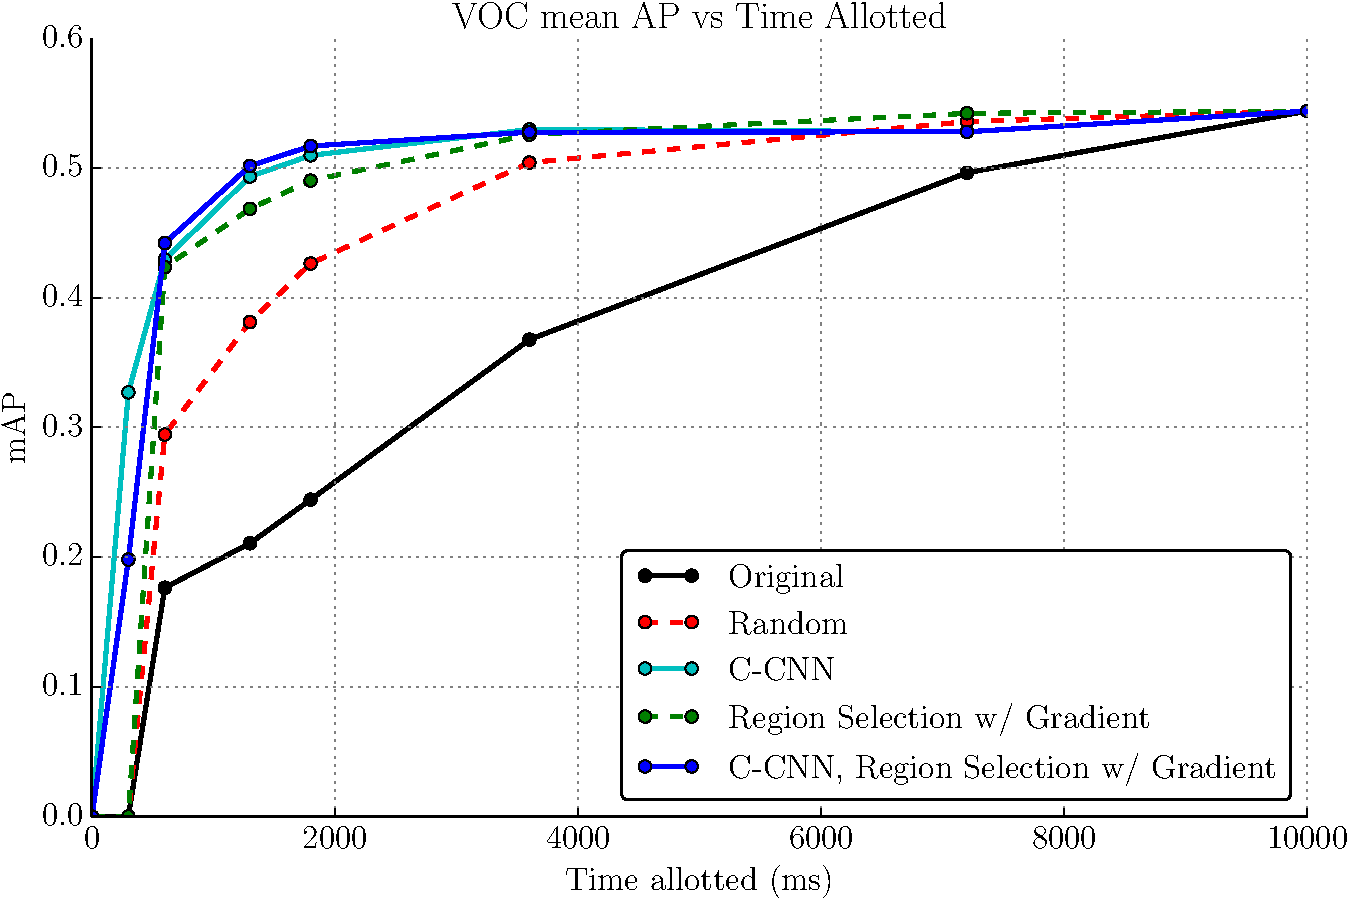
\includegraphics[width=.75\linewidth]{../ccnn/figures/_apvst_final.pdf}
    \caption{
Plotting Mean AP vs. Time Allotted allows comparison performance at a given time budget.
For example, at 1300 ms, random region selection gets about 0.42 mAP, while our best method (C-CNN with gradient-based region selection) obtains 0.50 mAP.
}\label{fig:apvst}
\end{subfigure}
\begin{subfigure}[b]{\linewidth}
    \centering
    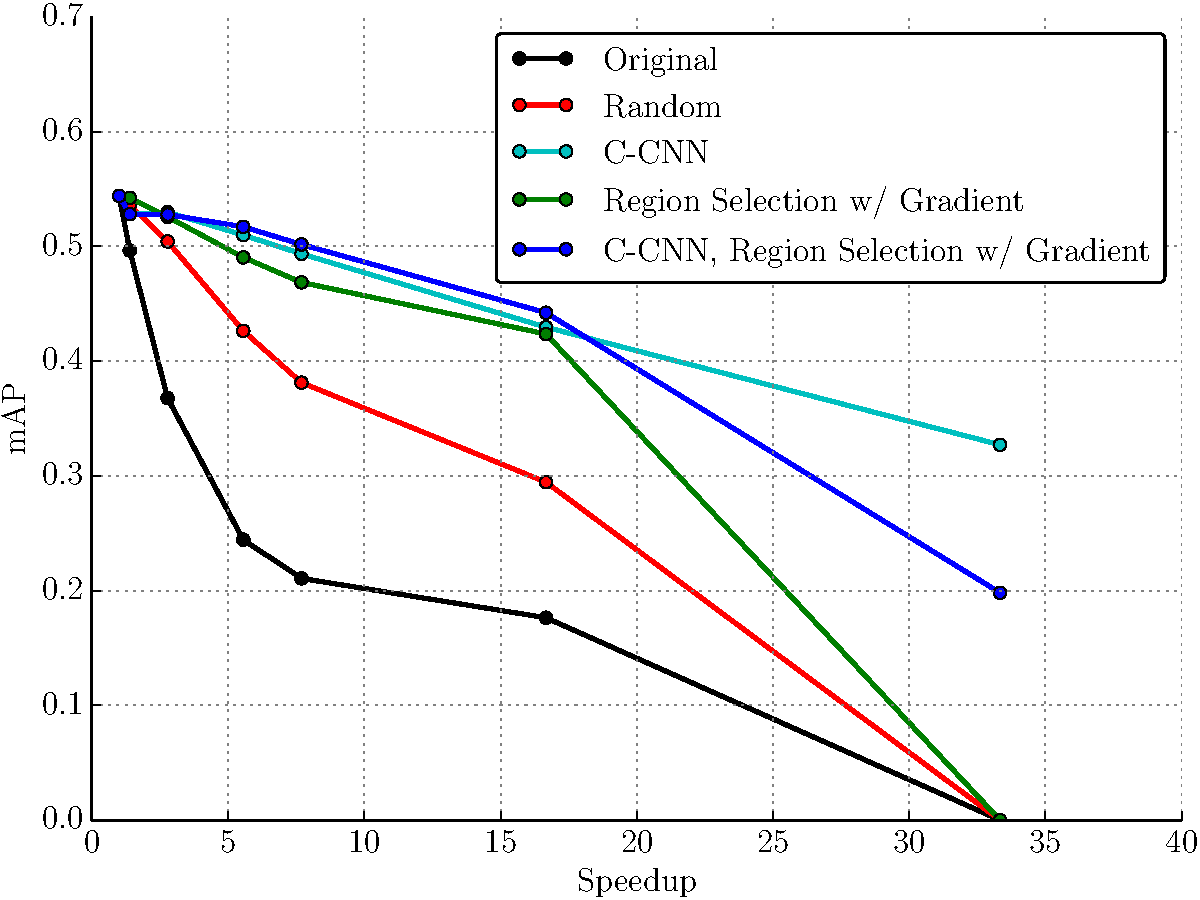
\includegraphics[width=.75\linewidth]{../ccnn/figures/_speedup_final_abs.pdf}
    \caption{
Plotting mean AP vs. speed-up factor allows comparison of speed-ups at a given mAP point.
For example, we can see that we should obtain mAP of 0.40 at around 20x speedup with our method.
}\label{fig:speedup}
\end{subfigure}
\caption{
Results of the Cascade CNN and other Anytime methods on the PASCAL VOC 2007 dataset.
}\label{fig:voc2007_results}
\end{figure}
